% AcademiX - Informe Entrega 2
% Compilar con pdfLaTeX.
\documentclass[letterpaper,10pt]{article}

\usepackage[left=1.25cm,right=1.25cm,top=1.1cm,bottom=1.1cm]{geometry}
\usepackage[utf8]{inputenc}
\usepackage[T1]{fontenc}
\usepackage[spanish,es-noshorthands]{babel}
\usepackage{helvet}
\usepackage{xcolor}
\usepackage{enumitem}
\usepackage{microtype}
\usepackage{graphicx}
\usepackage{tabularx}
\usepackage{longtable}
\usepackage{array}
\usepackage{multicol}
\usepackage{tikz}
\usepackage{hyperref}
\usepackage{booktabs}

\usetikzlibrary{arrows.meta,positioning,calc,shapes.geometric}

\definecolor{navy}{HTML}{18324F}
\definecolor{blue}{HTML}{2563EB}
\definecolor{teal}{HTML}{0F766E}
\definecolor{amber}{HTML}{B7791F}
\definecolor{green}{HTML}{15803D}
\definecolor{red}{HTML}{B91C1C}
\definecolor{line}{HTML}{CBD5E1}
\definecolor{soft}{HTML}{F8FAFC}
\definecolor{softblue}{HTML}{EFF6FF}
\definecolor{softteal}{HTML}{F0FDFA}
\definecolor{softamber}{HTML}{FFFBEB}
\definecolor{slate}{HTML}{475569}

\renewcommand{\familydefault}{\sfdefault}
\pagestyle{empty}
\setcounter{secnumdepth}{0}
\setlength{\parindent}{0pt}
\setlength{\parskip}{3pt}
\setlist[itemize]{leftmargin=*,topsep=1pt,itemsep=1pt,parsep=0pt}
\setlist[enumerate]{leftmargin=*,topsep=1pt,itemsep=1pt,parsep=0pt}
\hypersetup{colorlinks=true,urlcolor=navy,linkcolor=navy}
\emergencystretch=2em
\newcolumntype{Y}{>{\raggedright\arraybackslash}X}
\renewcommand{\arraystretch}{1.08}

\newcommand{\tagbox}[2]{\tikz[baseline=(n.base)]\node[rounded corners=2pt,fill=#1,inner xsep=5pt,inner ysep=2pt,text=white,font=\scriptsize\bfseries](n){#2};}
\newcommand{\sectionbar}[1]{\vspace{3pt}{\large\bfseries\color{navy}#1}\par\vspace{2pt}{\color{line}\hrule height 0.7pt}\vspace{3pt}}

\begin{document}

\begin{center}
{\LARGE\bfseries\color{navy} AcademiX: Entrega 2}\\
{\large Diseño preliminar, plan de desarrollo, riesgos y walking skeleton}\\
IIC3143 Desarrollo de Software · Equipo Lock In · Octubre 2026
\end{center}

\sectionbar{Resumen ejecutivo}

AcademiX es un LMS multi-tenant universitario enfocado en el flujo académico
crítico: cursos, secciones, módulos, material, quizzes, calificaciones,
publicación explícita de notas y auditoría. Esta entrega consolida el diseño
preliminar y reduce complejidad respecto de Entrega 1: se abandona la base de
datos por tenant y el Tenant Registry, reemplazándolos por PostgreSQL
compartida, \texttt{Institution} como tenant lógico e
\texttt{institution\_id} como frontera
de datos.

La arquitectura objetivo conserva robustez operacional: Railway como plataforma
de despliegue, réplicas de frontend/backend, PgBouncer, PostgreSQL HA y Railway
Bucket S3-compatible para material académico. El walking skeleton demuestra la
ruta de integración: frontend, backend, Docker, CI, Railway y release por tag.

\sectionbar{Trazabilidad contra pauta}

{\small
\begin{tabularx}{\textwidth}{p{3.2cm}p{2cm}Y}
\toprule
\textbf{Área pauta} & \textbf{Estado} & \textbf{Evidencia} \\
\midrule
Casos de uso actualizados & \tagbox{green}{Cubierto} & \texttt{03-use-cases-and-requirements.md}: CU-01 a CU-16 con actores, stakeholders, pre/postcondiciones, triggers, flujos y RNF. \\
Documento de diseño preliminar & \tagbox{green}{Cubierto} & Arquitectura, dominio, datos, walking skeleton y decisiones documentadas. \\
Arquitectura y demo/POC & \tagbox{green}{Cubierto} & \texttt{04-architecture.md}, \texttt{09-walking-skeleton-plan.md}, \texttt{11-cicd-evidence}. \\
Modelo de dominio & \tagbox{green}{Cubierto} & \texttt{05-domain-model.md} y \texttt{05-domain-model-uml.md}. \\
Modelo de datos & \tagbox{green}{Cubierto} & \texttt{06-data-model.md} y catálogo XLSX/CSV en \texttt{12-data-catalog.md}. \\
Plan de desarrollo & \tagbox{green}{Cubierto} & \texttt{08-work-plan.md}: siete semanas desde el lunes 5 de octubre de 2026. \\
Riesgos actualizados & \tagbox{green}{Cubierto} & \texttt{07-risks.md}: probabilidad, impacto, responsable, mitigación y contingencia. \\
PPT, informe y anexos & \tagbox{green}{Cerrado} & Informe, presentación Beamer, guía oral y anexos generados desde \texttt{docs/deliveries/2}. \\
\bottomrule
\end{tabularx}}

\sectionbar{Alcance funcional}

El MVP considera dos flujos principales: docente y estudiante. El docente
administra cursos, secciones, roles por \texttt{Enrollment}, módulos, material, quizzes
y libro de notas. El estudiante elige institución, accede a cursos autorizados,
consulta material publicado, responde quizzes y revisa notas publicadas.

Quedan fuera del MVP: administrador institucional, RBAC completo, rol
coordinador, IA, chat, calendario, workers, Redis, microservicios y entregas
manuales. La decisión evita que el diseño académico crezca más rápido que la
capacidad de implementación.

{\small
\begin{tabularx}{\textwidth}{p{2.5cm}Y}
\toprule
\textbf{Flujo} & \textbf{Casos de uso} \\
\midrule
Acceso & CU-01 elegir institución; CU-02 entrar al contexto institucional. \\
Cursos & CU-03 ver cursos y secciones; CU-04 gestionar secciones y roles. \\
Material & CU-05 publicar material; CU-06 consultar material; CU-14 organizar módulos. \\
Quizzes & CU-07 crear/publicar quiz; CU-08 responder; CU-09 enviar y calificar; CU-15 cancelar intento. \\
Notas & CU-10 configurar libro; CU-11 publicar; CU-12 ver notas; CU-16 revisar gradebook. \\
Auditoría & CU-13 consultar historial académico. \\
\bottomrule
\end{tabularx}}

\sectionbar{Arquitectura preliminar}

\begin{center}
\resizebox{0.95\textwidth}{!}{%
\begin{tikzpicture}[
  font=\sffamily\footnotesize,
  base/.style={draw=navy,thick,fill=softblue,rounded corners=3pt,align=center,inner sep=4pt,text width=2.7cm},
  ops/.style={draw=teal,thick,fill=softteal,rounded corners=3pt,align=center,inner sep=4pt,text width=2.8cm},
  data/.style={draw=amber,thick,fill=softamber,rounded corners=3pt,align=center,inner sep=4pt,text width=3cm},
  tenant/.style={draw=slate,thick,fill=white,rounded corners=2pt,align=center,inner sep=3pt,text width=2.3cm},
  fl/.style={-{Latex[length=1.8mm]},draw=navy,thick},
  repl/.style={-{Latex[length=1.8mm]},draw=amber,thick,dashed}
]
\node[base] (u) at (0,0) {\textbf{Usuarios}\\docente · estudiante\\ayudante};
\node[ops] (edge) at (3.5,0) {\textbf{Railway edge}\\load balancing};
\node[base] (fe) at (7,0.9) {\textbf{Next.js}\\frontend réplicas};
\node[base] (be) at (7,-0.9) {\textbf{NestJS}\\backend réplicas\\stateless};
\node[ops] (pool) at (10.6,-0.9) {\textbf{PgBouncer}\\connection pool};
\node[ops] (hap) at (14.1,-0.9) {\textbf{HAProxy}\\PostgreSQL HA};
\node[data] (dbp) at (17.8,-0.25) {\textbf{Primary}\\schema compartido};
\node[data] (dbr) at (17.8,-1.75) {\textbf{Replica}\\failover};
\node[data] (bucket) at (10.6,-3.05) {\textbf{Railway Bucket}\\PDF · presentaciones\\adjuntos};
\node[tenant] (uc) at (14.6,1.65) {Institution UC};
\node[tenant] (utfsm) at (17.6,1.65) {Institution UTFSM};
\node[tenant] (other) at (20.6,1.65) {Institution ...};
\coordinate (split) at (17.8,0.85);
\draw[fl] (u) -- (edge);
\draw[fl] (edge) -- (fe);
\draw[fl] (edge) -- (be);
\draw[fl] (fe) -- (be);
\draw[fl] (be) -- (pool);
\draw[fl] (pool) -- (hap);
\draw[fl] (hap) -- (dbp);
\draw[repl] (dbp) -- node[right,font=\scriptsize]{streaming} (dbr);
\draw[fl] (be) |- (bucket);
\draw[fl] (dbp.north) -- (split);
\draw[fl] (split) -| (uc.south);
\draw[fl] (split) -- (utfsm.south);
\draw[fl] (split) -| (other.south);
\end{tikzpicture}}

\footnotesize Figura 1. Arquitectura objetivo: Railway, réplicas de aplicación,
pooling, PostgreSQL HA, object storage y separación lógica por
\texttt{institution\_id}.
\end{center}

La decisión central separa dos preocupaciones. La continuidad operacional se
aborda con réplicas, healthchecks, PgBouncer, PostgreSQL HA, backups y PITR. El
aislamiento de datos se aborda con \texttt{Institution}, autorización
contextual, queries scopeadas, \texttt{institution\_id}, FK compuestas,
constraints y auditoría.

{\small
\begin{tabularx}{\textwidth}{p{3.1cm}YY}
\toprule
\textbf{Falla} & \textbf{Respuesta esperada} & \textbf{Límite} \\
\midrule
Réplica frontend/backend & Railway balancea hacia réplicas sanas. & Requiere más de una réplica. \\
Backend completo & Restart policy y rollback si corresponde. & Un bug global requiere corrección. \\
Primary PostgreSQL & PostgreSQL HA promueve una réplica y HAProxy redirige. & Conexiones en vuelo deben reintentar. \\
Mala migración/corrupción & Backups y PITR. & HA no corrige errores lógicos replicados. \\
Object storage & Core sin archivos puede seguir. & Cargas/descargas fallan temporalmente. \\
Proveedor/región & Riesgo aceptado del MVP. & No se implementa multi-cloud. \\
\bottomrule
\end{tabularx}}

\sectionbar{Modelo de dominio}

\begin{center}
\resizebox{0.95\textwidth}{!}{%
\begin{tikzpicture}[
  font=\sffamily\scriptsize,
  entity/.style={draw=navy,fill=soft,rounded corners=3pt,minimum width=2.45cm,minimum height=0.8cm,align=center},
  core/.style={draw=teal,fill=softteal,rounded corners=3pt,minimum width=2.45cm,minimum height=0.8cm,align=center},
  grade/.style={draw=amber,fill=softamber,rounded corners=3pt,minimum width=2.45cm,minimum height=0.8cm,align=center},
  arr/.style={-{Latex[length=1.5mm]},draw=slate,thick}
]
\node[entity] (u) at (0,1.6) {User};
\node[entity] (im) at (3.4,1.6) {InstitutionMembership};
\node[entity] (i) at (6.8,1.6) {Institution};
\node[core] (c) at (10.2,1.6) {Course};
\node[core] (s) at (13.6,1.6) {Section};
\node[core] (e) at (13.6,0.25) {Enrollment};

\node[core] (m) at (10.2,-1.1) {CourseModule};
\node[core] (mat) at (6.8,-1.1) {Material};
\node[grade] (q) at (13.6,-1.1) {Quiz};
\node[grade] (qa) at (17.0,-1.1) {QuizAttempt};

\node[grade] (gi) at (10.2,-2.45) {GradeItem};
\node[grade] (g) at (13.6,-2.45) {Grade};
\node[entity] (a) at (17.0,-2.45) {AuditEvent};
\draw[arr] (u) -- (im);
\draw[arr] (im) -- (i);
\draw[arr] (i) -- (c);
\draw[arr] (c) -- (s);
\draw[arr] (s) -- (e);
\draw[arr] (c) -- (m);
\draw[arr] (m) -- (mat);
\draw[arr] (m) -- (q);
\draw[arr] (q) -- (qa);
\draw[arr] (q.south) -- ++(0,-0.38) -| (gi.north);
\draw[arr] (gi) -- (g);
\draw[arr] (g) -- (a);
\end{tikzpicture}}

\footnotesize Figura 2. Dominio resumido del MVP.
\end{center}

\texttt{Enrollment} es el pivote académico: indica quién pertenece a qué curso
y sección, en qué institución y con qué rol (\texttt{teacher},
\texttt{assistant}, \texttt{student}). No se modela coordinador ni RBAC
completo. \texttt{GradeItem} representa una columna del libro de notas;
\texttt{Grade} representa la nota concreta de un estudiante para
ese ítem.

\sectionbar{Modelo de datos}

El modelo usa una sola PostgreSQL compartida y un schema evolutivo. Las tablas
globales son \texttt{institutions}, \texttt{users} e
\texttt{institution\_memberships}. Las entidades académicas son tenant-owned y
llevan \texttt{institution\_id}.

{\small
\begin{tabularx}{\textwidth}{p{2.2cm}p{4cm}Y}
\toprule
\textbf{Categoría} & \textbf{Tabla} & \textbf{Descripción} \\
\midrule
Global & \texttt{institutions} & Tenant lógico: slug, nombre, estado y ciclo de vida. \\
Global & \texttt{users} & Identidad global reutilizable entre instituciones. \\
Acceso & \texttt{institution\_memberships} & Habilita acceso de usuario a institución. \\
Curso & \texttt{courses}, \texttt{sections} & Curso semestral y separación lógica por sección. \\
Curso & \texttt{enrollments} & Une usuario, institución, curso, sección y rol académico. \\
Contenido & \texttt{course\_modules}, \texttt{materials} & Organización del material común visible para secciones del curso. \\
Evaluación & \texttt{quizzes}, \texttt{quiz\_attempts} & Quiz con preguntas JSONB e intentos estudiantiles. \\
Notas & \texttt{grade\_items}, \texttt{grades} & Columnas del libro y notas concretas por estudiante. \\
Auditoría & \texttt{audit\_events} & Historial inmutable de cambios sensibles. \\
\bottomrule
\end{tabularx}}

El catálogo de datos se adjunta como XLSX/CSV e incluye tablas, columnas,
tipos, PK/FK, nulabilidad y descripciones.

\sectionbar{Walking skeleton y CI/CD}

El walking skeleton valida riesgos técnicos de integración antes de construir
el flujo académico completo. La evidencia incluye frontend Next.js, backend
NestJS, \texttt{GET /health}, Dockerfiles, GitHub Actions, configuraciones Railway y
release por tag.

\begin{center}
\begin{tabular}{ccc}
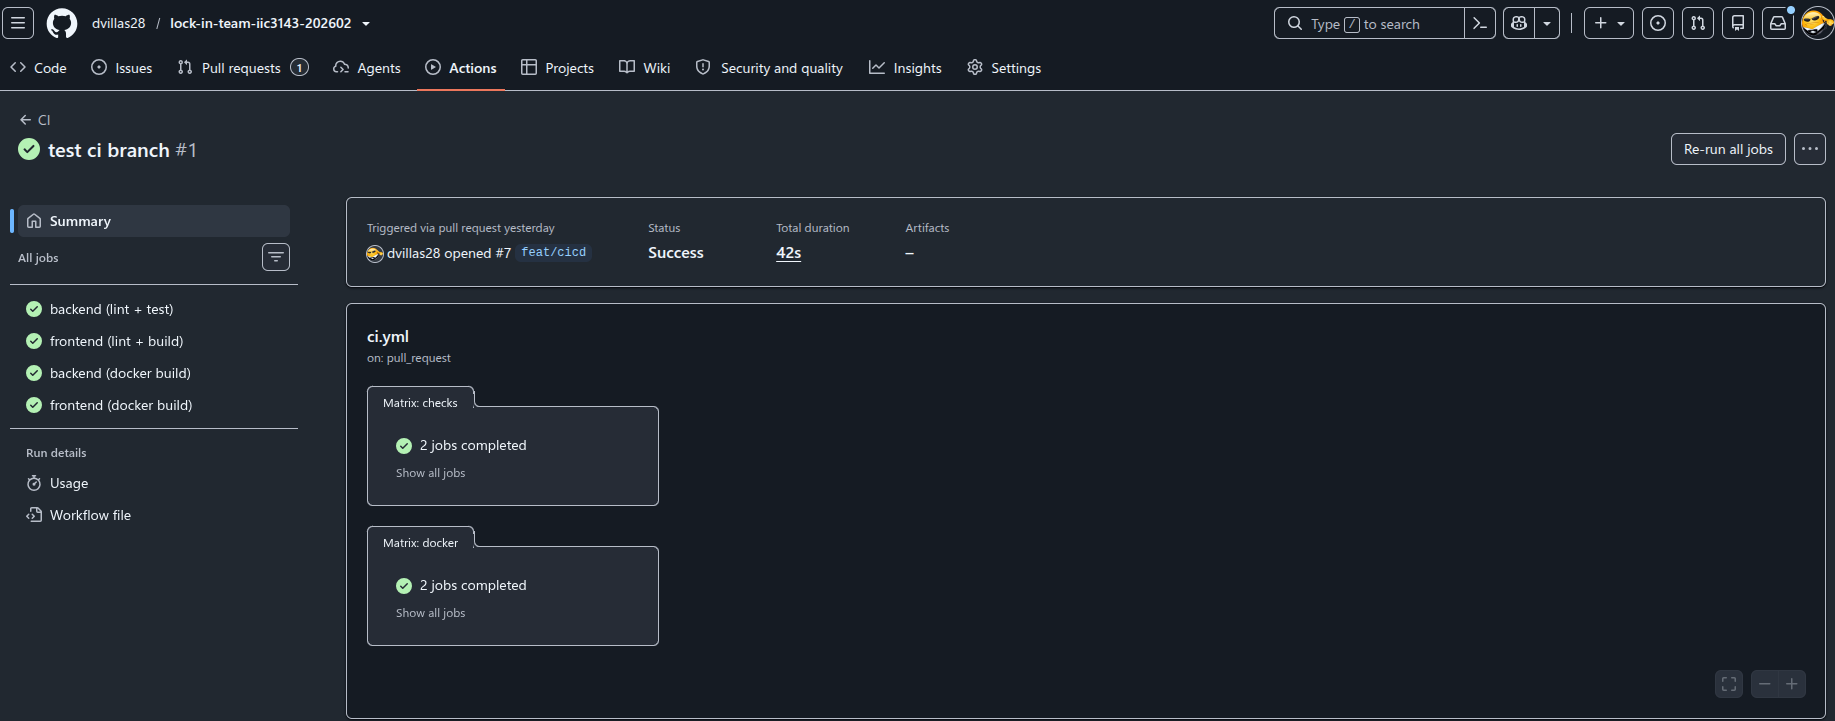
\includegraphics[width=0.29\textwidth]{../11-cicd-evidence/img/03-ci-run.png} &
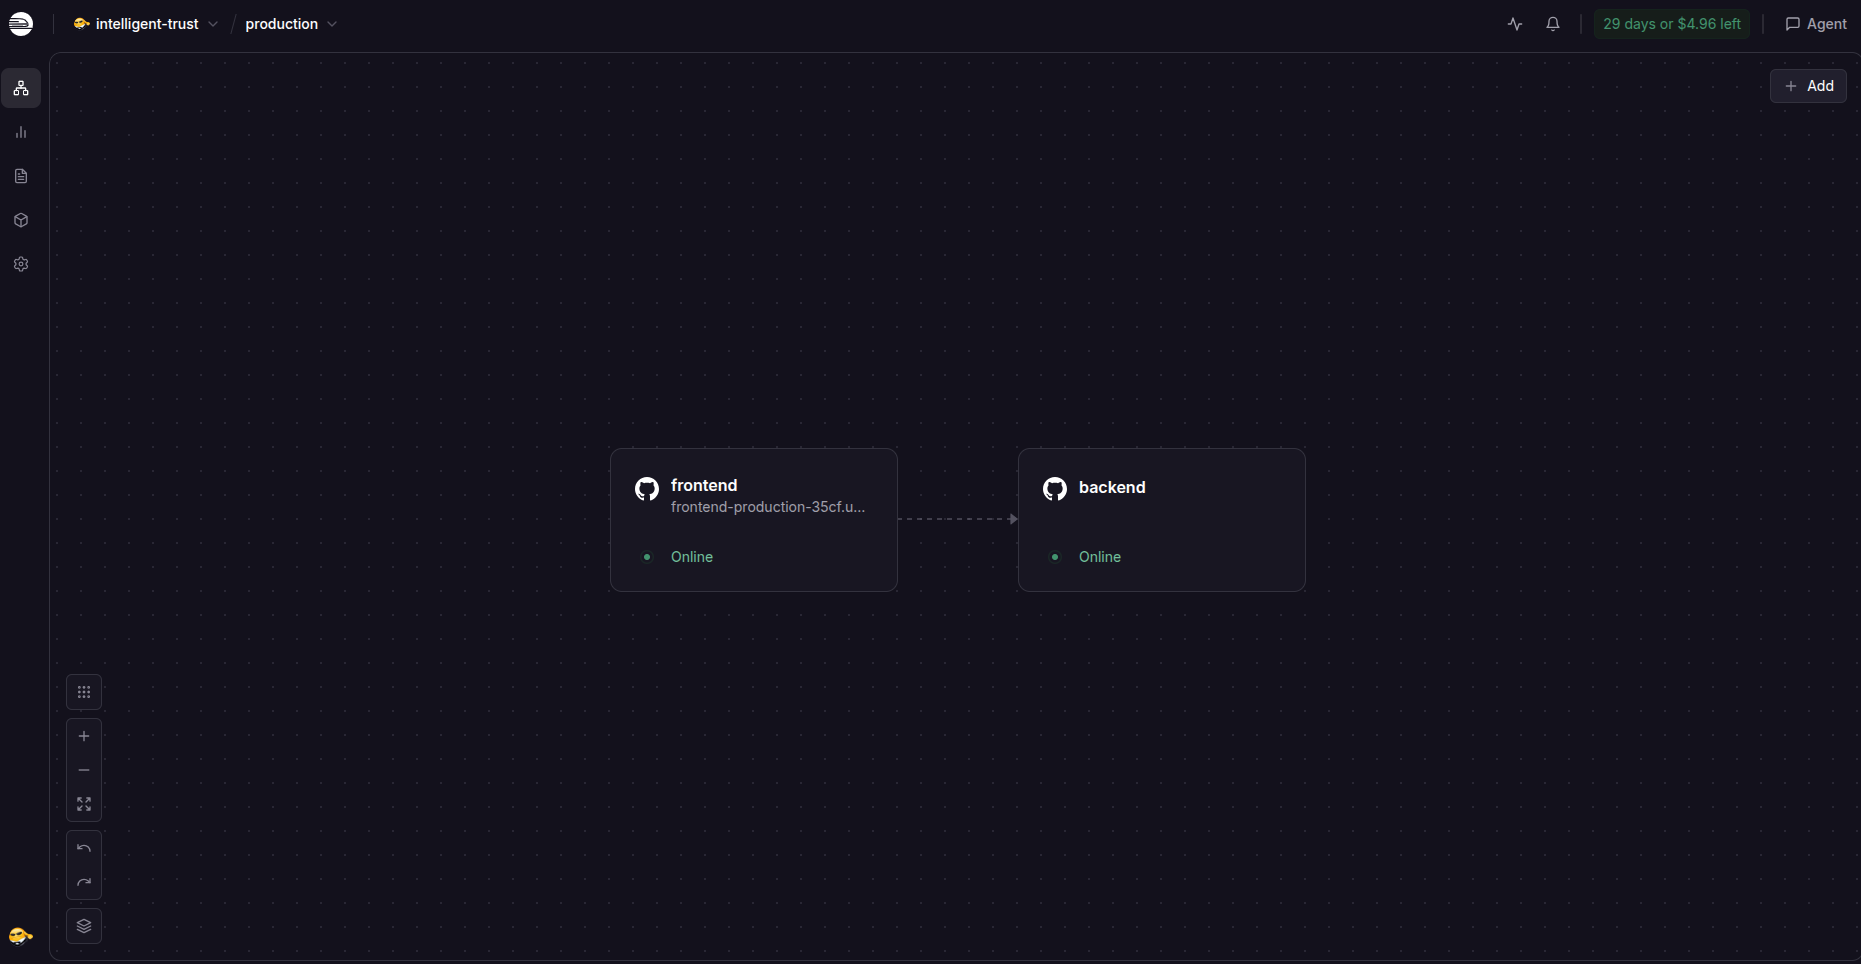
\includegraphics[width=0.29\textwidth]{../11-cicd-evidence/img/06-railway-project.png} &
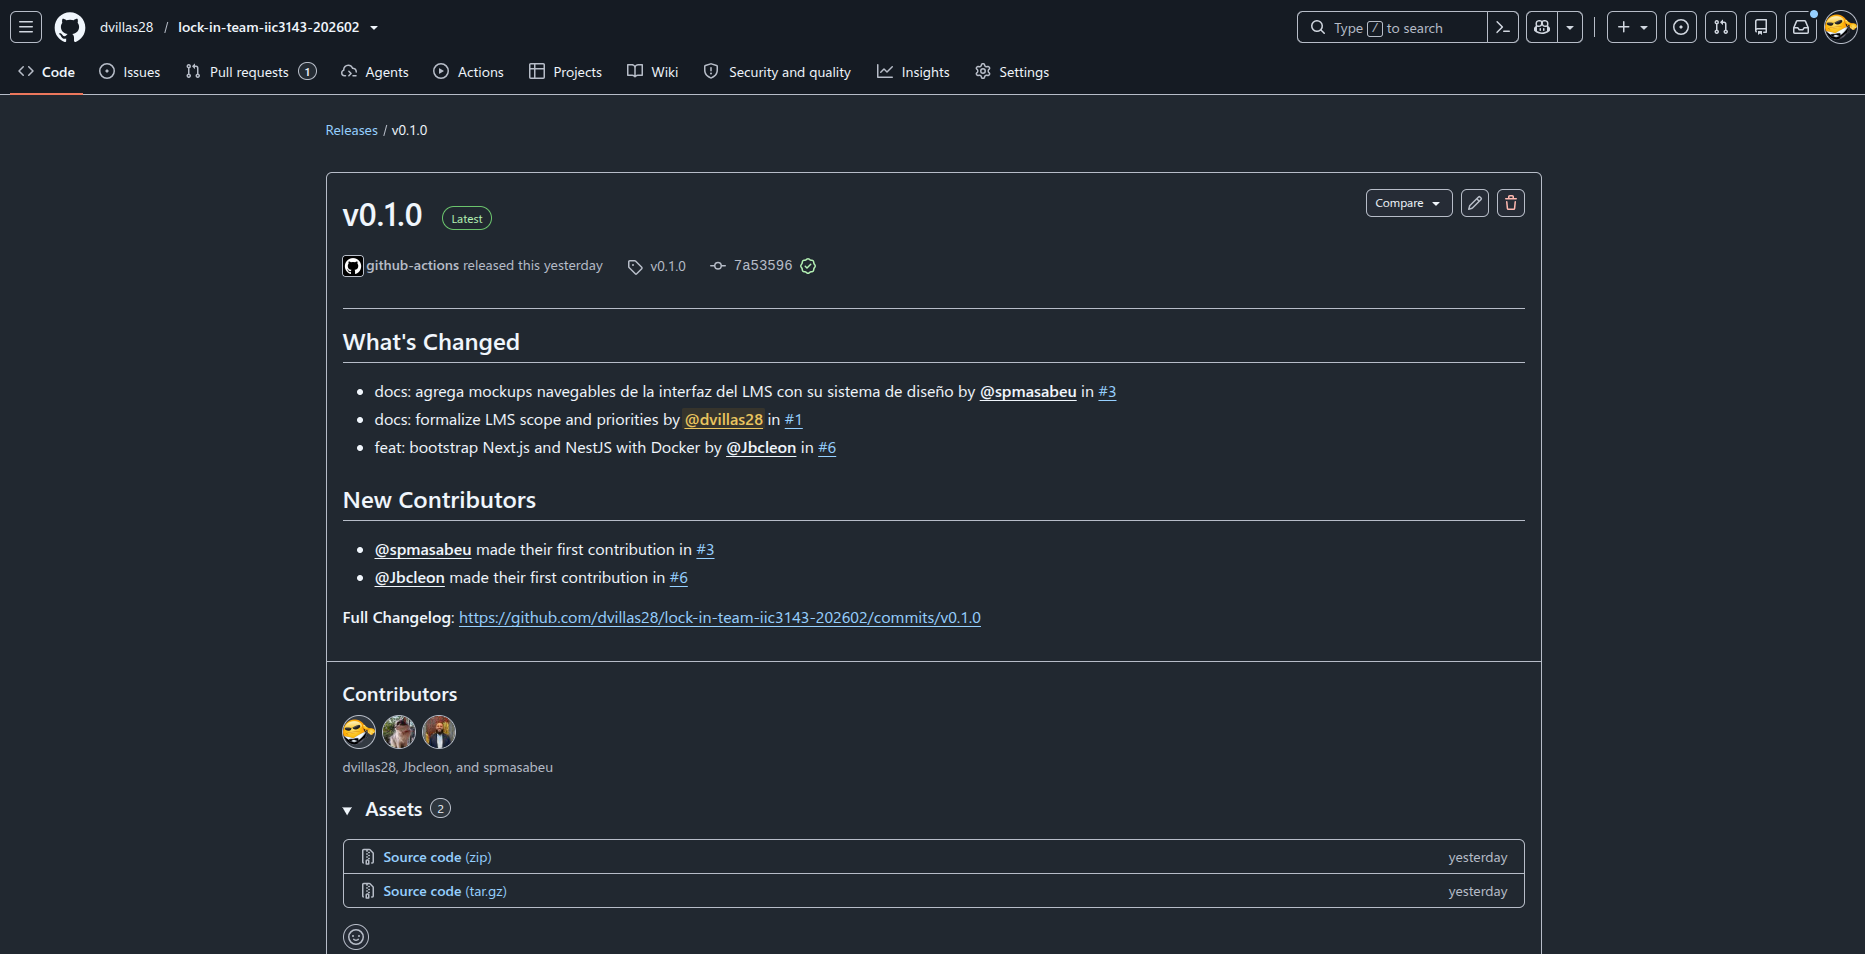
\includegraphics[width=0.29\textwidth]{../11-cicd-evidence/img/11-github-release.png} \\
\footnotesize CI ejecutado & \footnotesize Railway & \footnotesize GitHub release \\
\end{tabular}
\end{center}

\sectionbar{Plan de desarrollo}

El plan parte el lunes 5 de octubre de 2026 y cubre siete semanas. Daniel
Fierro aborda el bot PR reviewer; Sebastián Palma backend e infraestructura;
Julián Contreras y Matías frontend; Daniel Villaseñor CI/CD, Scrum Master y
gestión.

{\small
\begin{tabularx}{\textwidth}{p{1cm}p{2.4cm}Yp{3cm}}
\toprule
\textbf{It.} & \textbf{Fechas} & \textbf{Foco} & \textbf{Responsables} \\
\midrule
1 & 2026-10-05 a 2026-10-11 & Plan ejecutable, CI/CD, contrato y presentación. & Villaseñor, Palma \\
2 & 2026-10-12 a 2026-10-18 & PostgreSQL compartida e identidad institucional. & Palma \\
3 & 2026-10-19 a 2026-10-25 & Contexto institucional y aislamiento. & Palma, Fierro \\
4 & 2026-10-26 a 2026-11-01 & Cursos, secciones, roles y shell frontend. & Palma, Contreras, Matías \\
5 & 2026-11-02 a 2026-11-08 & Módulos, material y quizzes. & Contreras, Matías, Palma \\
6 & 2026-11-09 a 2026-11-15 & Notas, publicación, auditoría y PR reviewer. & Palma, Fierro, Frontend \\
7 & 2026-11-16 a 2026-11-22 & Hardening, release, documentación y ensayo. & Todo el equipo \\
\bottomrule
\end{tabularx}}

\sectionbar{Riesgos actualizados}

La planilla de riesgos concentra riesgos técnicos y de gestión con responsable,
probabilidad, impacto, mitigación y contingencia. Los riesgos más importantes
son fuga entre Institutions, queries sin scope institucional, sobrealcance,
auditoría incompleta, CI/CD que no refleje el estado real y presentación final
demasiado densa.

{\small
\begin{tabularx}{\textwidth}{p{1.1cm}p{3.1cm}p{2.5cm}Y}
\toprule
\textbf{ID} & \textbf{Riesgo} & \textbf{Responsable} & \textbf{Mitigación} \\
\midrule
R-01/R-02 & Fuga o query sin scope institucional & Sebastián Palma & Contexto centralizado, FK institution-aware y tests UC/UTFSM. \\
R-09/R-10 & Railway o CI/CD mal configurado & Daniel Villaseñor & Healthchecks, Docker reproducible, pipelines y release por tag. \\
R-12 & Sobrealcance funcional & Daniel Villaseñor & Recorte al flujo curso-material-quiz-notas. \\
R-13 & Auditoría incompleta & Sebastián Palma & AuditEvent en misma transacción y tests de cambios sensibles. \\
R-15 & Frontend permite acciones fuera de rol & Julián Contreras, Matías & UI derivada de permisos; backend conserva autorización final. \\
R-16 & Bot PR reviewer genera ruido & Daniel Fierro & Activación gradual y revisión humana obligatoria. \\
\bottomrule
\end{tabularx}}

\sectionbar{Conclusión}

La Entrega 2 deja una base estable para construir: casos de uso trazados,
arquitectura defendible, modelo de dominio, modelo de datos, plan de trabajo,
riesgos y walking skeleton. La simplificación frente a Entrega 1 no elimina
garantías críticas; elimina complejidad prematura y conserva las defensas que
importan: aislamiento tenant-aware, autorización contextual, auditoría,
CI/CD reproducible y operación con HA/pooling/storage.

\sectionbar{Anexos declarados}

Los anexos de la carpeta \texttt{docs/deliveries/2} incluyen catálogo de datos XLSX,
CSV de tablas/columnas/constraints, OpenAPI, capturas CI/CD, evidencia Railway,
riesgos completos y plan de desarrollo detallado.

\end{document}
